\chapter{Introduction}

\section{Who Was Kowalevski?}
\begin{wrapfigure}{i}{0.25\textwidth}
\centering
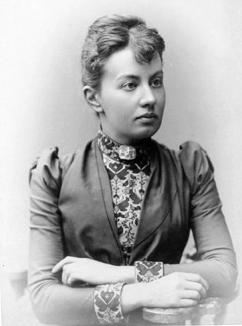
\includegraphics[width=0.25\textwidth]{kovalevskaya_8}
\end{wrapfigure}

Sofya Vasilyevna Kovalevskaya (1850-1891) was a Russian mathematician. For various reasons, including the theorem at the center of this discussion, she remains one of the most significant female figures in the history of this discipline.

First of all, it is important to note that from here on, we will often refer to her by the name she used to sign her publications, namely Kowalevski.

To leave Russia, she had to enter into a marriage of convenience; she married a man with whom she did not have any real emotional relationship and from whom she was often geographically distant. This allowed her to continue her studies in Germany, where she met Karl Weierstrass, one of the most influential mathematicians of his time. After their initial meeting in the professor's study, their relationship continued to develop thanks to Kowalevski's evident mathematical talents, which Weierstrass could not help but nurture. In fact, he continued to give her private lessons, eventually supervising her research work.

Regarding Kowalevski's political ideas, we can historically assert her closeness to feminist movements and socialist and radical ideas, which can be traced back to her family background and the insights she gained from her experiences in the states of modern Europe. It is certainly noteworthy that she received several copies of radical magazines of that time from her sister Anna, which discussed the so-called ancient nihilism\footnote{For ancient nihilists, science, rather than religion and superstition, appeared to be the most effective means of helping the population, thus representing truth and progress.}.

However, our focus is not on her political, social, and philosophical ideas, but rather on her contributions to mathematics. With the help of what we might call her mentor, Kowalevski made several important discoveries. After several years of collaboration, she published three doctoral theses in a single year, 1874. But this is not the only notable aspect; she was also the first woman to earn a doctorate, which was made possible by Weierstrass's support, as evidenced by a letter he wrote to Fuchs, a colleague at the University of Berlin, regarding the approval of Kowalevski's theses. Additionally, her publications, significant in their own right, proved to be milestones in mathematics. Specifically, the topics addressed are:
\begin{itemize}
\item Partial Differential Equations (PDE), Cauchy-Kowalevski theorem
\item Mechanics, Kowalevski top
\item Elliptic integrals
\end{itemize}

After the success, crowned by some awards that naturally followed the publication of these researches, she returned to Russia for a period; however, this choice proved to be futile for the continuation of her academic career. Subsequently, when the husband who had enabled her to study in Germany passed away, she moved to Sweden, where she achieved another milestone: she became the first woman in the world to be a professor of mathematics, obtaining the chair at the University of Stockholm.

Unfortunately, her life was cut short prematurely at the age of 41 by pneumonia, which, according to sources, prevented her from pursuing her great passion: literary production. Although she could not express herself as she wished in this field, there are numerous artistic representations of her, both in literature and cinema.

The main cinematic works are:
\begin{itemize}
\emergencystretch 3em
\item \textit{Sofya Kowalevski}(1985, Lenfilm, 3 episodes, 218 minutes), Ayan Gasanovna Shakhmaliyeva (1932-1999, originally from Azerbaijan).

\item \textit{A Hill on the Dark Side of the Moon} (Swedish: \textit{Berget på månens baksida})(1983), Lennart Hjulström (1938-2022)
\end{itemize}

The main literary works are:
\begin{itemize}

\item an autobiography: \textit{A Russian Childhood} (1978, Springer New York, NY), Sofya Kovalevskaya, translated and edited by Beatrice Stillman

\item a biography: \textit{Sonja Kovalevsky. What I Experienced with Her and What She Told Me About Herself} (1982, Ed. Albert Bonniers, Stockholm), Anne Charlotte Leffler (a close friend of Kowalevski, sister of the mathematician Gösta Mittag-Leffler and wife of the Italian algebraist Pasquale del Pezzo)

\item a biography: \textit{Little Sparrow: A Portrait of Sophia Kovalevsky} (1983, Ohio University Press, Athens, Ohio), Don H. Kennedy

\item a biographical novel: \textit{Beyond the Limit: The Dream of Sofya Kovalevskaya} (2002, Tom Doherty Associates, LLC), Joan Spicci (mathematician and educator)

\item a biographical short story: \textit{Too Much Happiness}\footnote{the story recounts the last days of Kowalevski's life, enriched by reminiscences of the past that Munro acquired from letters, diaries, and writings (documents accessed through Don H. Kennedy's wife, who is a distant descendant of Kowalevski)}
(2009, Harper's Magazine), Alice Munro (1931-2024, Nobel Prize in Literature)

\end{itemize}

\section{The Cauchy-Kowalevski Theorem}

Having introduced the historical figure, we can now take the first step towards the discovery of one of Kowalevski's researches: the Cauchy-Kowalevski theorem, which we will abbreviate as TCK from here on.

\emergencystretch 3em
First, let us quickly describe the scientific context of that time related to PDEs.

The father of this research carried out in the 19th century is Augustin-Louis Cauchy, a mathematician who will surely be familiar to the reader. During those years, particularly between 1835 and 1842, Cauchy was engaged in developing the theory of holomorphic functions, already initiated by other prominent figures such as Euler, Laplace, and Fourier.

Cauchy had the intuition to apply these results to differential equations.

It is important to grasp, trying to immerse ourselves in the mindset of that period, that classical theory and power series were very promising tools, primarily for their simplicity and elegance, but also for the approximation potential that a simple truncation of a series encapsulated.

Cauchy's attempt to apply the tools obtained from his research to differential equations was successful but only partially so for a simple reason: he could not go beyond the study of ordinary differential equations (ODEs) and linear PDEs.

The leap was made thanks to Kowalevski and Weierstrass. The latter was very optimistic about the results he thought could be achieved, perhaps even more so than Cauchy: consider that he formulated a conjecture that it would be possible to define analytic functions through differential equations, thanks to formal power series derived from the expressions of the equations. For this reason, he pushed Kowalevski, along with her talent, towards this topic, in which she was able to investigate much more deeply.

However, it is wrong to think that Kowalevski's guides were only Cauchy and Weierstrass: other mathematicians dedicated themselves to these topics, among whom we remember, among the most important, Briot, Bouquet, and Fuchs, who better developed the concepts of singularities, and Jacobi, who first provided the definition of an equation in normal form\footnote{this, in particular, will prove to be a crucial concept in Kowalevski's research}.

Based on these foundations, Kowalevski's important idea can be summarized as follows:
\begin{enumerate}
\item implement a variable change that allowed writing a nonlinear equation in normal form (see chapters \ref{tools} and \ref{invariant} for the meaning of this term), maintaining the regularity assumptions on the data, and dealing with the existence of a solution to this system;
\item transform any equation in normal form into a particular quasi-linear system;
\item apply the majorant method already used by Cauchy for his discoveries on ODEs and linear PDEs.
\end{enumerate}
As often happens in mathematics, the proof was later simplified by E. Goursat in his mathematical analysis textbook around 1900. Moreover, over time, more abstract and general statements and proofs were proposed, thanks to the work of Ovsyannikov, Treves, and Nirenberg.

We quickly note that Darboux also achieved results very similar to Kowalevski's, but with less generality, in the same period; in fact, both published their research in 1874.

In light of what has been said so far, we pose some crucial questions, to which we want to find the most exhaustive answers possible and which will guide the discussion we will address:
\begin{itemize}
\item is it possible for an analytic solution to exist for a system of PDEs with Cauchy data?
\end{itemize}
if so
\begin{itemize}
\item under what assumptions?
\item is it unique?
\item is the resulting problem well-posed?
\item what applications do the obtained results have?
\end{itemize}